\documentclass[class=report,crop=false, 12pt]{standalone}
\usepackage[screen,nosolutions]{../myscratch}
%\usepackage[screen]{../myscratch}

\begin{document}


\titre[S]{Premiers pas}
%===============================

\insertvideo{onJG9sLbtNE}{Premiers pas -- Activité 1}

\insertvideo{4rdLxPcYMZ4}{Premiers pas -- Activité 2}

\insertvideo{jK29YG6WPgw}{Premiers pas -- Activité 3}

\bigskip
\bigskip


\begin{activite}

Commençons par déplacer le chat Scratch.

\begin{enumerate}
  \item
  \begin{itemize}
    \item Commence par déposer le bloc \og quand le drapeau vert est cliqué \fg{} sur la partie droite.
    \item Puis colle juste au-dessous de ce bloc, le bloc \og avancer de 10 pas\fg{}.
    \item Clique plusieurs fois sur le drapeau vert. 
  \end{itemize}

Scratch devrait avoir avancé !

\begin{center}
  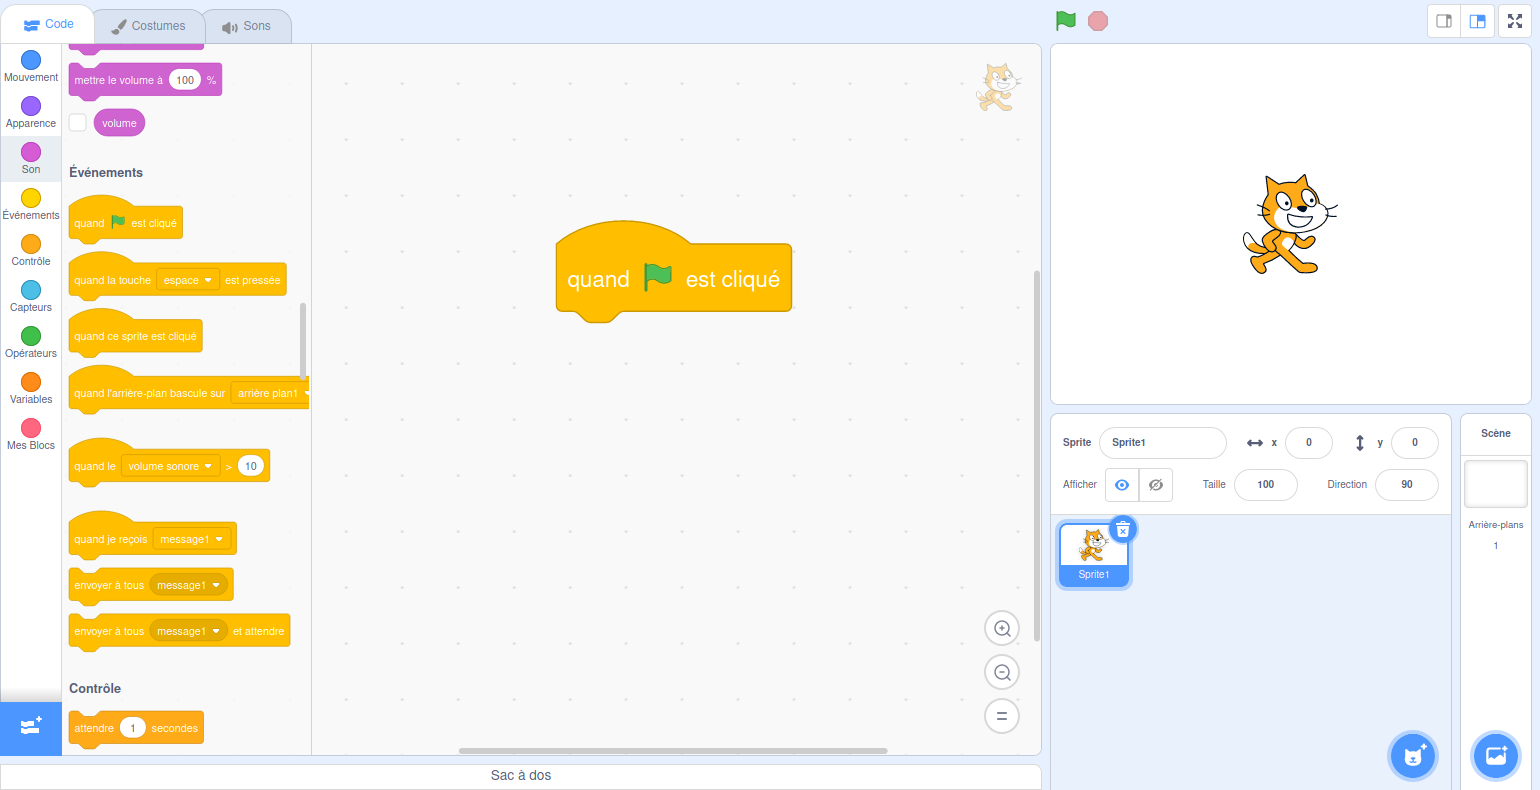
\includegraphics[width=0.65\textwidth]{ecran-01-ex1a}

  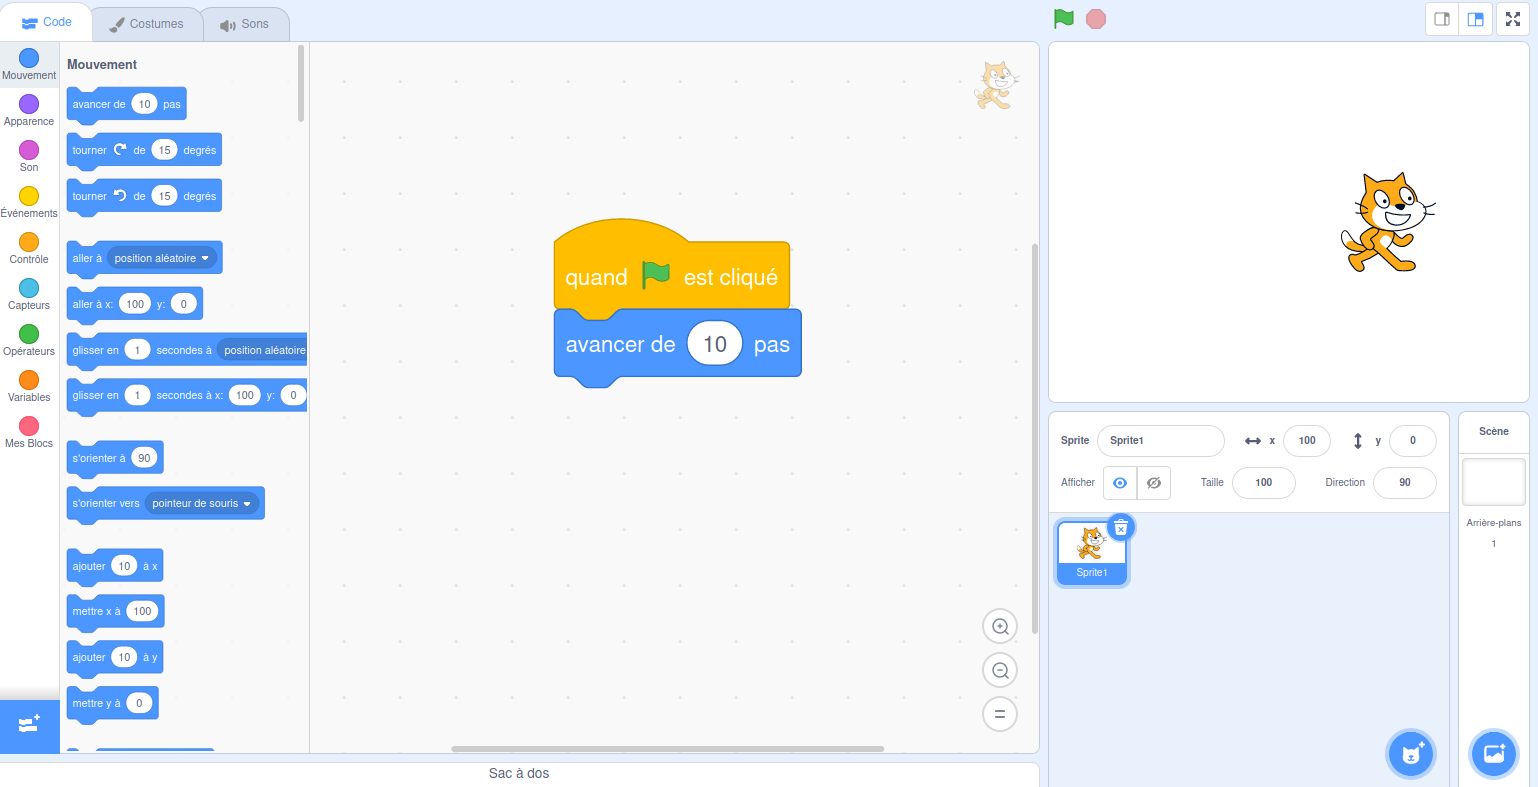
\includegraphics[width=0.65\textwidth]{ecran-01-ex1b}
\end{center}  
  



Les deux blocs à positionner :
\begin{center}
\begin{scratch}
  \blockinit{quand \greenflag est cliqué}
\end{scratch}
\qquad\qquad
\begin{scratch}
  \blockmove{avancer de \ovalnum{10} pas}
\end{scratch}
\end{center}    
  
  Il y a plusieurs problèmes : Scratch finit par être coincé à droite de l'écran, on aimerait qu'il revienne au départ, on aimerait aussi tracer son chemin.
  
  
  \item Pour que tout le monde démarre dans la même position à chaque fois que le drapeau vert est cliqué, commence toujours par les blocs suivants avant d'ajouter tes propres instructions :
  
  \begin{itemize}
    \item Quand le drapeau vert est cliqué
    \item Aller à $x = 0$, $y = 0$
    \item S'orienter à 90\textdegree\ (vers la droite)
    \item Effacer tout
    \item Stylo en position d'écriture
  \end{itemize}  

\medskip

Tu auras besoin des blocs \og{}Stylo\fg{}. Voici comment y accéder.
\begin{center}
\small
\begin{minipage}{0.45\textwidth}
\center
\myfigure{0.5}{
\tikzinput{ecran-01-styloaa}
} 

\emph{1. En bas à gauche, clique sur \og{}Ajouter une extension\fg{}.}
\end{minipage}
\begin{minipage}{0.45\textwidth}
\center
\myfigure{0.5}{
\tikzinput{ecran-01-stylobb}
} 

\emph{2. Choisis l'extension \og{}Stylo\fg{}.}
\end{minipage}

\myfigure{0.5}{
\tikzinput{ecran-01-stylocc}
} 

\emph{3. Tu as maintenant les blocs \og{}Stylo\fg{} à disposition.}
%\end{minipage}

\end{center}

Positionne ces blocs, puis fais maintenant avancer Scratch de $100$ pas ! 

\begin{center}
\begin{scratch}
  \blockinit{quand \greenflag est cliqué}
  \blockmove{aller à x: \ovalnum{0} y: \ovalnum{0}}
  \blockmove{s'orienter à \ovalnum{90}}
  \blockpen{effacer tout}
  \blockpen{stylo en position d'écriture}
\end{scratch}
\end{center} 
  

  

  \item Voici ton premier programme :
  \begin{itemize}
    \item Fais avancer Scratch de 50 pas
    \item Fais une pause d'une seconde
    \item Fais encore avancer Scratch de 50 pas, puis une pause
    \item Fais avancer Scratch de 50 pas une dernière fois
  \end{itemize}
  
\myfigure{0.9}{
\tikzinput{ecran-01-ex1}
} 

  
\end{enumerate}
 
\end{activite}




\begin{activite}

Trace la figure suivante représentant la lettre \og G \fg{}.

\begin{center}
\begin{minipage}{0.3\textwidth}
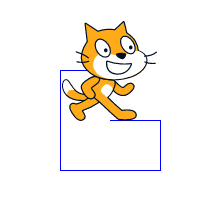
\includegraphics[width=\textwidth]{ecran-01-ex2}
\end{minipage}
\begin{minipage}{0.3\textwidth}
\myfigure{0.5}{
\tikzinput{ecran-01-ex2a}
} 
\end{minipage}
\begin{minipage}{0.3\textwidth}
\begin{scratch}
  \blockmove{s'orienter à \ovalnum{0}}
  \blockspace[0.5]
  \blockmove{s'orienter à \ovalnum{180}}
  \blockspace[0.5]
  \blockmove{s'orienter à \ovalnum{90}}
  \blockspace[0.5]
  \blockmove{s'orienter à \ovalnum{-90}}
\end{scratch}
\end{minipage}
\end{center}

Utilise seulement des blocs \og avancer \fg{} et des blocs \og s'orienter à ... \fg{} pour te diriger vers le haut ($0$\textdegree), vers le bas ($180$\textdegree), vers la droite ($90$\textdegree) ou vers la gauche ($-90$\textdegree). Tu peux insérer des pauses afin d'avoir le temps de visualiser correctement chaque mouvement.

\bigskip

\textbf{Bonus.} 
Si tu es motivé, trace le symbole \og arobase \fg{}  \at :
\myfigure{1}{
\tikzinput{ecran-01-ex2b}
} 
 
\end{activite}


\begin{activite}

Trace la figure suivante réprésentant la lettre \og L \fg{}.

\begin{center}
\begin{minipage}{0.3\textwidth}
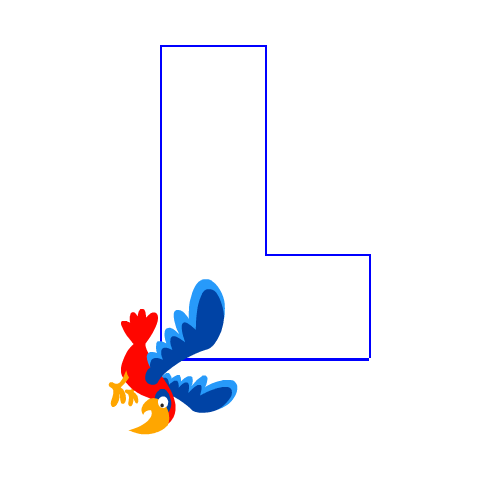
\includegraphics[width=\textwidth]{ecran-01-ex3}
\end{minipage}
\begin{minipage}{0.3\textwidth}
\myfigure{0.5}{
\tikzinput{ecran-01-ex3a}
} 
\end{minipage}
\begin{minipage}{0.3\textwidth}
\begin{scratch}
  \blockmove{tourner \turnright{} de \ovalnum{90} degrés}
  \blockspace[1]
  \blockmove{tourner \turnleft{} de \ovalnum{90} degrés}
\end{scratch}
\end{minipage}  
\end{center} 

Utilise seulement les blocs \og avancer \fg{} et \og tourner vers la droite de $90$\textdegree \fg{} pour tourner d'un quart de tour à droite, ou le bloc \og tourner vers la gauche de $90$\textdegree \fg{} pour tourner d'un quart de tour à  gauche. Tu peux insérer des pauses afin d'avoir le temps de visualiser correctement chaque mouvement.

\bigskip

\textbf{Bonus 1.} Dans l'onglet \og Costumes \fg{}, choisis l'apparence que tu veux donner au lutin.

\textbf{Bonus 2.} Si tu as le temps, trace le symbole d'un point d'interrogation.


\myfigure{1}{
\tikzinput{ecran-01-ex3b}
} 

\end{activite}


\ifx \displaysolutions \myzero
\else
\begin{code}
\setscratch{scale=\scalesolution}
\onesolution{Premiers pas}{Activité 1}{
\begin{scratch}
  \blockinit{quand \greenflag est cliqué}
  \blockmove{aller à x: \ovalnum{0} y: \ovalnum{0}}
  \blockmove{s'orienter à \ovalnum{90}}
  \blockpen{effacer tout}
  \blockpen{stylo en position d'écriture}
  \blockmove{avancer de \ovalnum{50} pas}  
  \blockcontrol{attendre \ovalnum{1} secondes} 
  \blockmove{avancer de \ovalnum{50} pas}  
  \blockcontrol{attendre \ovalnum{1} secondes} 
  \blockmove{avancer de \ovalnum{50} pas}  
\end{scratch}
}
\onesolution{Premiers pas}{Activité 2}{
\begin{scratch}
  \blockinit{quand \greenflag est cliqué}
  \blockmove{aller à x: \ovalnum{0} y: \ovalnum{0}}
  \blockmove{s'orienter à \ovalnum{90}}
  \blockpen{effacer tout}
  \blockpen{stylo en position d'écriture}
  \blockmove{avancer de \ovalnum{50} pas}  
  \blockcontrol{attendre \ovalnum{1} secondes} 
  \blockmove{s'orienter à \ovalnum{180}}
  \blockmove{avancer de \ovalnum{50} pas}  
  \blockcontrol{attendre \ovalnum{1} secondes} 
  \blockmove{s'orienter à \ovalnum{-90}}
  \blockmove{avancer de \ovalnum{100} pas}  
  \blockcontrol{attendre \ovalnum{1} secondes} 
  \blockmove{s'orienter à \ovalnum{0}}
  \blockmove{avancer de \ovalnum{100} pas}  
  \blockcontrol{attendre \ovalnum{1} secondes} 
  \blockmove{s'orienter à \ovalnum{90}}
  \blockmove{avancer de \ovalnum{50} pas}  
\end{scratch}
}
\onesolution{Premiers pas}{Activité 3}{
\begin{scratch}
  \blockinit{quand \greenflag est cliqué}
  \blockmove{aller à x: \ovalnum{0} y: \ovalnum{0}}
  \blockmove{s'orienter à \ovalnum{90}}
  \blockpen{effacer tout}
  \blockpen{stylo en position d'écriture}

  \blockmove{avancer de \ovalnum{100} pas} 
  \blockcontrol{attendre \ovalnum{1} secondes} 
  \blockmove{tourner \turnleft{} de \ovalnum{90} degrés}

  \blockmove{avancer de \ovalnum{50} pas} 
  \blockcontrol{attendre \ovalnum{1} secondes} 
  \blockmove{tourner \turnleft{} de \ovalnum{90} degrés}
  \blockmove{avancer de \ovalnum{50} pas} 
  \blockcontrol{attendre \ovalnum{1} secondes} 
  \blockmove{tourner \turnright{} de \ovalnum{90} degrés}
  \blockmove{avancer de \ovalnum{100} pas} 
  \blockcontrol{attendre \ovalnum{1} secondes} 
  \blockmove{tourner \turnleft{} de \ovalnum{90} degrés}
  \blockmove{avancer de \ovalnum{50} pas} 
  \blockcontrol{attendre \ovalnum{1} secondes} 
  \blockmove{tourner \turnleft{} de \ovalnum{90} degrés}
  \blockmove{avancer de \ovalnum{150} pas} 
 \end{scratch}
}
\end{code}
\fi



\end{document}


